\def\pilot{{\tt PILOT}}
\def\RR{{\tt SAIL}}
\def\bb{\noindent\hspace{.46cm}$\bullet$\hspace{.19cm}}




\documentclass[10pt]{article}

\usepackage{graphicx}
\usepackage{wrapfig}
\usepackage[most]{tcolorbox}


%\usepackage{simplemargins}
%\setallmargins{1in}

\usepackage{url}
\evensidemargin -.2cm
\oddsidemargin -.2cm
\setlength\topmargin{-0.7in}
\setlength{\textwidth}{16cm}   % width of body
\setlength{\textheight}{9.2in}   % heigth of body
%\setlength{\sectionskip}{2ex}
\setlength{\itemsep}{-1in}
\setlength{\leftmarginii}{.05in}

\newcommand{\ve}[1]{{\em #1}} % venue of publication
\newcommand{\ti}[1]{``#1''} % title of publication
\newcommand{\lmt}{(limited to period starting 01/2013)}

\newcommand{\todo}[1]{\textcolor{red}{TODO: #1}}

\begin{document}


%\pagestyle{empty}

\begin{center}
{\Large \bf Candidate Statement\\
\smallskip
{\large \bf Mihai Surdeanu}}
\end{center}
%\smallskip

\begin{wrapfigure}{r}{0.45\textwidth}
  \begin{center}
    \vspace{-10mm}
    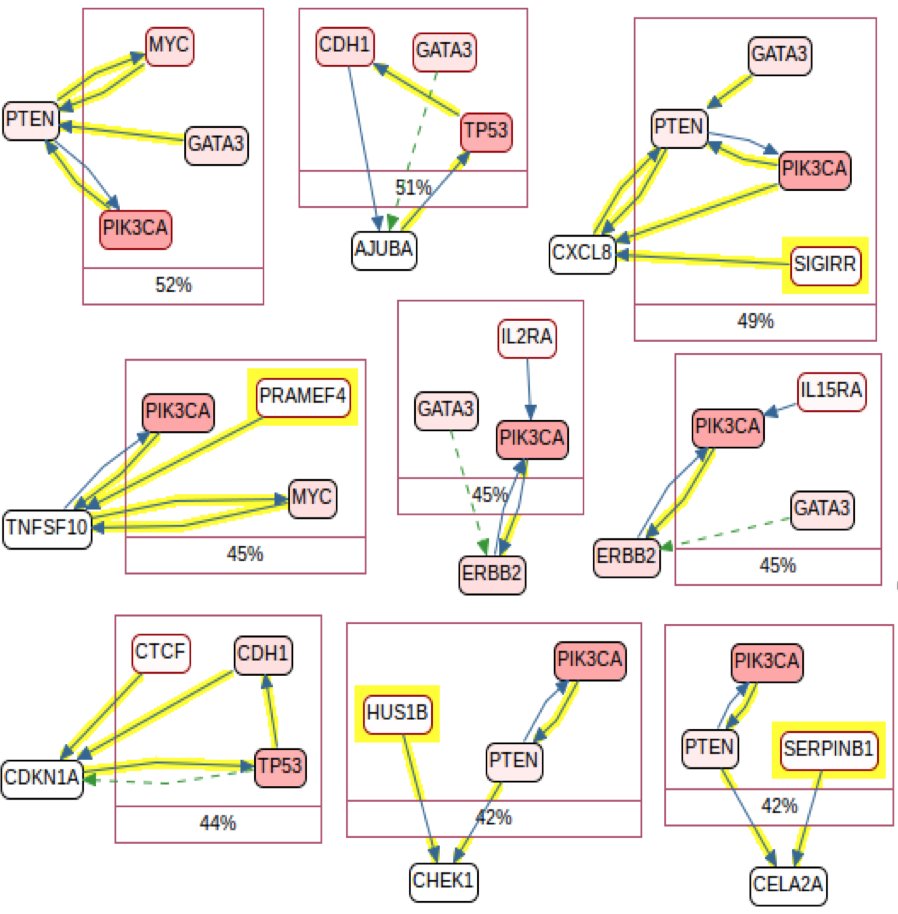
\includegraphics[width=0.40\textwidth]{mutex_simplified}
  \end{center}
  \vspace{-4mm}
  \caption{{\small A collection of protein signaling pathways that impact breast cancer. Each box illustrates a group of signaling pathways that share a downstream target protein, where each target is known to drive breast cancer. For example, the top left box shows three signaling pathways activating the PTEN protein. 
  A personalized cancer treatment adressing any  given target must block \emph{all} signaling pathways to that protein in order to succeed.
  % otherwise the disease switches in time from a blocked pathway to an unblocked one. 
  Importantly, the information highlighted in \colorbox{yellow!30}{yellow} shows novel pathways discovered by our machine reading approach, which help explain actual patient data, and were missed by domain experts that curated cancer literature. We observed similar results for 11 different cancer types.}}
  \label{fig:mutex}
  \vspace{-10mm}
\end{wrapfigure}


\section{Research Accomplishments}

My research is on semantic models for natural language, that is, getting computers to understand human language. This is an important challenge: it is estimated that up to 80\% of the web content is unstructured information, including text.\footnote{{\scriptsize \url{http://www.computerweekly.com/blog/CW-Developer-Network/IBM-80-percent-of-our-global-data-is-unstructured-so-what-do-we-do}}}
This happens in domain-specific scenarios as well.
For example, PubMed, a repository and search engine for biomedical literature,\footnote{{\scriptsize \url{https://www.ncbi.nlm.nih.gov/pubmed}}} indexes more than 1 million scientific publications each year. This is clearly beyond the human processing capacity.  
My work focuses on turning these vast amounts of data into knowledge. 
For example, Figure~\ref{fig:mutex} shows one of the outcomes of my work: in collaboration with a cancer researcher,\footnote{Emek Demir, Oregon Health \& Science University} we\footnote{Unless otherwise specified, plural first-person pronouns refer to my collaborators and I, where collaborators come mostly from the lab I have built at UA.} showed that the machine reading of research literature yields novel hypotheses for the understanding and treatment of multiple cancers [87]. 

Two important research threads, which often overlap, are pervasive in my work. First, I focus on {\em interpretable} models for natural language processing (NLP).
That is, methods that transform what computers understand of human text into human-consumable/communicable knowledge.
%That is, I aim to open the black box of machine learning (ML) by developing NLP models that are understandable by their human users. 
Second, I am interested in {\em natural language inference}, a stepping stone towards building machines that can reason over text, by ``understanding bigger things from knowing smaller parts''\footnote{{\scriptsize \url{http://mitp.nautil.us/article/170/last-words-computational-linguistics-and-deep-learning}}} that were extracted from text.

I detail these two directions below. 

\subsection*{Interpretable Models for NLP}

% I define interpretability here from the human perspective: can the human understand what the machine learns? 
I believe the interpretability of NLP models (i.e., can the human understand what the machine learns?)
 is a key, necessary property for the wide acceptance of artificial intelligence (AI), and for the transformation of AI into a collaborator in the acquisition and use of human knowledge. 
For example, in the medical domain, an AI system that answers treatment questions would not be trusted if 
the treatment recommendation is not explained in terms that can be understood by the doctor and the patient. Further, interpretability  reduces the cost of maintaining NLP/ML systems, especially in our inter-disciplinary context, where the systems that we build are likely to be used, debugged, and maintained by domain experts (e.g., cancer researchers) who are not NLP/ML specialists. 

In my work, I have approached the goal of interpretability from multiple perspectives:

{\flushleft {\bf Rule-based models}}: We have shown that rule-based approaches, where decisions are made based on a series of deterministic operations, lead to interpretable models (i.e., models that can be interpreted and edited by humans) that obtain state-of-the-art performance for many NLP tasks, including event extraction [46], coreference resolution [3, 6, 33], and bioinformatics [87, 23]. We have released Odin, an open-source platform  for the development of grammars for information extraction that includes a novel language and runtime environment [23, 54]. One key feature of Odin is that rules written for different representations of content (e.g., over surface tokens, or over syntactic dependencies) can coexist in the same grammar, which increases the grammar's robustness to incorrect syntax. 
As a simple example, Odin may capture that a protein is phosphorylated through the direct object of the verb {\em phosphorylate}, or from the phrase following the verb in text (when syntax fails). 
This, together with other features such as simplicity and interpretability of the rule language, and efficient runtime, made Reach, our bioinformatics system built on top of Odin,\footnote{{\scriptsize \url{https://github.com/clulab/reach}}} the most widely used machine reading system in the DARPA Big Mechanism program.\footnote{Most cancer modeling groups in the program use Reach, including Harvard Medical School, Oregon Health and Science University, University of Pittsburgh, SRI.}
%\footnote{A large number of Github issues reporting bugs or feature requests for Reach come from computational biologists, demonstrating again the importance of interpretability.}

{\flushleft {\bf Learning rules}}: The main drawback of rule-based approaches is the high cost of manually developing rules. To mitigate this, we have worked on automated rule learning. 
For example, we have proposed a bootstrapping approach for knowledge acquisition that combines the recent advances in neural networks with the interpretability of rules. Starting from only a few examples, our approach learns dense representations (or embeddings) for both extraction rules and the concepts to be extracted [88]. We have shown that this achieves state-of-the-art performance, and, importantly, can be exported into a decision-list model with minimal performance loss (by keeping the extraction rules whose embedding vectors are closest to the average embedding for a given class to be learned). 
For example, our algorithm learns that {\em said {\tt @ENTITY}} and {\em President {\tt @ENTITY}} are good rules to extract person names, and {\em {\tt  @ENTITY} government} is a good rule to extract nationalities ({\tt @ENTITY} is a placeholder for the actual name to be extracted).
%
In the space of supervised learning (i.e., where sufficient training examples are available), we have proposed an approach that ``snaps to grid'' a probabilistic, feature-based model by converting features to rules, and simplifying the model statistics into votes assigned to each rule. 
% We have shown that this strategy looses some performance (less than 10\%, relative) from the probabilistic model, but the resulting model can be understood and edited by human domain experts. The resulting interpretable model, after human experts correct obvious errors, 
We have shown that the resulting model can be understood and modified by human domain experts, and, ultimately, achieves the same performance as the probabilistic one [55].  

{\flushleft {\bf  Learning models that explain themselves}}: 
Last but not least, I have developed methods for learning models that can accomplish a task but also explain themselves using natural language.
% Last but not least, I have worked on models that jointly learn how to solve the task at hand, and how to explain themselves using natural language text. 
For example, we have proposed a question answering (QA) model that both identifies correct answers and produces compelling human-readable justifications for why those answers are correct [4]. % We demonstrated that this joint approach outperforms other approaches for both tasks. 
We implemented this idea using a latent-variable perceptron, where the answer justification is modeled as a latent variable. In more recent work, we have introduced a deep learning architecture with max-pooling that outperforms the latent-variable perceptron model [89]. 
For example, our deep learning model answers the question {\em ``Scientists use ice cores to help predict the impact of
future atmospheric changes on climate. Which property of ice cores do these scientists use?''} with the answer {\em ``The composition of ancient materials trapped in air bubbles''} and it explains it with the sentence: {\em ``Ice cores: cylinders of ice that scientists use to study trapped atmospheric gases and particles frozen with in the ice in air bubbles.''}


\subsection*{Natural Language Inference}

The NLP community has made tremendous progress towards extracting atomic facts from text such as who are the agents and patients for a given action [12, 43, 80, inter alia], or extracting binary relations between named entities such as {\tt date\_of\_birth}  [29, 66, 68, inter alia].
However, the task of compositionality in NLP models, i.e., how we combine these smaller facts into ``bigger things'', remains an important challenge. This prevents us from building better NLP applications such as more effective search engines that are capable of answering complex questions. 
For example, while search engines can answer queries such as {\em ``Barack Obama birth date''}, the difficulty of compositionality prevents them from answering more complex questions such as {\em ``What conditions allow Northern Lights near the Equator?''}

I have addressed this challenge using several different approaches:

{\flushleft {\bf Aligning semantic structures}}: In my previous work on QA, we have proposed to repurpose statistical alignment models traditionally used for machine translation to align semantic structures such as predicate-argument frames between questions and their answers. We have shown that this approach learns robust QA strategies that answer complex questions even when their  answers have minimal word overlap with the question [9, 39]. 
For example, our approach learns that {\em ``Salt and pepper the grouse \ldots Pan-fry it in a little olive oil \ldots pour in a little white wine''} is a good answer to the question {\em ``How can I cook a grouse with normal household spices?''}
In more recent work, we have shown how training data for these alignment models can be efficiently generated by exploiting the discourse structure of text (e.g., we generate an artificial question and answer training example from a pair of clauses, where one clause elaborates the information in the other) [21]. This strategy facilitates the development of complex QA models when no training data is available.

{\flushleft {\bf Higher-order lexical semantic models}}: One limitation of the above approach is that it can only capitalize on direct evidence seen in training (i.e., pairs of aligned questions and answers) to build associations between semantics in the question and the answer. 
To address this limitation, we proposed a QA model that can take advantage of indirect evidence, i.e., indirect associations that are never observed during training.
Our approach implements a higher-order formalism that allows lexical semantic models (both alignment models and word embeddings) to chain direct evidence to construct indirect associations between question and answer texts, by casting the task as the traversal of graphs that encode direct term associations. 
For example, our approach understands that the text {\em ``Zoe's Diner has great pancakes.''} is a good answer to the question {\em ``Where should we go for breakfast?''} by assembling an inference that links {\em breakfast} $-$ {\em pancakes} and {\em pancakes} $-$ {\em hashbrowns}.
We showed that such an approach improves the QA performance of several lexical semantic models that capture only direct associations [5].

{\flushleft {\bf Learning to aggregate explanations}}: Lastly, we recently introduced a QA model that learns how to jointly identify correct answers and produce human-readable answer explanations. The explanations are aggregated from multiple sentences extracted from textual knowledge bases  [4]. We showed that information aggregation for answer explanation is key to addressing the information need in complex questions.
For example for the science question {\em ``Which organism is a producer?''} with correct answer {\em grass}, our approach assembles a two-sentence explanation, where each sentence comes from a different resource: {\em ``Producer is an organism that produces its own food and is food for other organism; usually a green plant. Grass is a green, leafy plant that often covers the ground.''}

\subsection*{Future Work}

To date, my work has % been well-received in the NLP community. It has led
led to publications in top NLP conferences (ACL, EMNLP, NAACL, EACL, COLING, CoNLL, etc.) and top journals (Computational Linguistics, Transactions of the Association of Computational Linguistics, Journal of Artificial Intelligence Research, etc.). Four of these conference papers were among the top three most cited papers at their respective venues [26, 29, 33, 46].\footnote{Statistics from \scriptsize \url{https://aminer.org/conferencebestpapers}} 
The NLP systems we have developed have placed in the top three at seven international NLP evaluations [65, 8, 72, 76, 1, 84, 85].
Lastly, my work has directly led or contributed to the creation of two NLP companies. 

Looking forward, I will:
\begin{itemize}
\item Address grand challenges with a tangible impact in our society. For example, we will continue our work on mining for undiscovered cancer treatments using automated reading and assembly of research literature [87]. Further, we will work on disease prevention by analyzing social media and mining for correlations between social media activity and risk of diseases such as type 2 diabetes mellitus or other diseases impacted by lifestyle choices [24, 90].
\item Continue to lead inter-disciplinary efforts at University of Arizona. I currently lead several such efforts at UA, all of which will be expanded in the future: I lead a collaboration with the School of Information (SI) and the Molecular and Cellular Biology department on the above cancer research project;
I lead a joint effort between CS and the Nutritional Sciences department on disease prevention using social media analysis; I will be part of the leadership team (representing NLP) in UA's new data science center ({\small \url{http://d7.arizona.edu}}); and lastly, I collaborate with the College of Nursing and the SI on a NIH-sponsored project to identify important events in electronic health records.
\item Aim to be among the leaders of NLP efforts at UA. For example, I started and continue to manage a NLP reading group that grew into a campus-wide effort. We now routinely host 20 -- 30 participants per meeting, from multiple departments across campus: CS, Linguistics, School of Information, MIS, Psychology, Speech, Language, and Hearing Sciences, as well as former UA graduates that work in relevant industries in Tucson. 
I have designed 500/600 level courses where students participated in international NLP challenges such as the Fake News Challenge ({\small \url{http://www.fakenewschallenge.org}}) and the Allen AI Science Challenge ({\small \url{https://www.kaggle.com/c/the-allen-ai-science-challenge}}).
\item Build open-source software systems that are used by many. For example, our bioinformatics system ({\small \url{https://github.com/clulab/reach}}) is used by many groups internationally. Similarly, our NLP/ML library ({\small \url{https://github.com/clulab/processors}}) is becoming one of the most popular NLP packages for the Scala language. I contributed to Stanford's CoreNLP library ({\small \url{https://stanfordnlp.github.io/CoreNLP/}}), which has been downloaded tens of thousands of times. 
\item Continue to work on fundamental research issues. For example, I plan to model compositionality for natural language inference using reinforcement learning. Such an approach for QA would learn how to assemble the explanations that lead to the correct answers, using the final goal of identifying the correct answer as the only form of supervision. Further, I plan to work on transforming neural networks, which are opaque, into interpretable models. 
% For interpretable models, I plan to continue working on combining representation learning with interpretability, by extending it with other important linguistic phenomena such as sense disambiguation (e.g., by having a different representation for each sense of the concepts to be learned). 
\end{itemize}

\section{Teaching Accomplishments}

\subsection*{Contributions to Course Development}

When I started at UA there were limited opportunities for students interested in NLP. The only NLP course offered at the time was Statistical Natural Language Processing, in Linguistics. While this is a great course, it is not sufficient to cover the entire field of NLP. 
%In particular, this course covers only some of the machine learning (ML) models used in NLP, and does not address at all the building of end-to-end NLP applications. 
To address these curriculum limitations, I created two courses in my first two years at UA: ISTA 456/556 Text Retrieval and Web Search, which focuses on information retrieval (this course has been renumbered as CSC 483/583), and ISTA 455/555 Applied Natural Language Processing, which is designed as a continuation of the Statistical NLP course, emphasizing the development of complete, end-to-end NLP applications.  Additionally, I contributed to the development of ISTA 116, a foundational course that is fundamental to students interested in NLP.

More recently, I contributed to the creation of a single landing page for NLP at UA (\url{http://nlp.arizona.edu}), so students have an immediate understanding of the availability of NLP faculty on campus. The next step is to create a unified NLP curriculum. For this, I will work together with the Human Language Technology program in Linguistics\footnote{I currently hold a courtesy appointment in Linguistics.} and the other faculty listed in the website above to make sure that the courses we design and teach complement well the courses currently offered. For example, I have recently designed a course called Algorithms for Natural Language Processing, which will cover more modern algorithms for NLP that are not covered in the Statistical Natural Language Processing course such as recurrent neural networks.

\subsection*{Teaching Principles}

As a teacher, I explore new ways of presenting the material in order to emphasize the big picture behind the material covered. Showing how the fundamental principles covered in the subject matter impact real life (e.g., smarter search engines due to natural language understanding; novel disease treatments due to big data analysis) engages the students, and gives them a glimpse of where they could potentially use the material in a real-world career.

A second focus of my teaching work is personalization of information dissemination. 
I have personalized the learning experience in my courses or laboratories through customizable assignments and projects. This allows students to choose a preferred learning path that emphasizes either practice, or theory, or both.
I also believe that teaching is not a one-way process. I prefer to receive continuous feedback from students (either through comments during class or a series of ungraded quizzes) about the quality of my teaching and of the course materials. In the past few years I have a included an informal teacher and course evaluation (TCE) quiz that students take mid semester. This helps me adjust the delivery of the course to the students currently taking it. This is important especially for NLP courses, which tend to be attended by students from multiple departments, with various backgrounds. 

Last but not least, I aim to further improve engagement through active learning. My preferred method is through course projects that tackle important issues. For example, the course project for the Text Retrieval and Web Search course in Spring 2017 is the Fake News Challenge (\url{http://www.fakenewschallenge.org}). We approach these projects top down, e.g., Why is the detection of fake news important?; How would you tackle it intuitively?; What knowledge do we need to actually implement these ideas? I have found this strategy to engage students considerably more than passively teaching about NLP and ML. 

As a result of applying these teaching principles, I have received consistently high TCEs in my teaching activity at UA, with a score usually over 4.5/5 on my teaching effectiveness, the rating of the course, and usefulness of lecture and other materials. 

\subsection*{Research Mentoring} 

I have taught students to maintain a high-level perspective on their research. Students should always be able to answer a few questions about their research: What problem are you trying to solve? What is your contribution? How would you present this in a paper? 

I am a hands-on adviser to students at all levels: undergraduate, MS, PhD, postdoctoral. I regularly help students with their code. I continue to code, and continue to be one of the main contributors to our public software projects, which helps me be up to date on software development, and provide relevant practical feedback. I encourage students to approach me with any issues, ranging from theory to coding questions: I have an open-door policy in addition to regular one-hour weekly meetings. 

Further, I believe it is important for students to publish their work as early as possible and be exposed to their research community by attending conferences, reviewing papers, etc. This not only exposes them to other relevant work, but it forces students to learn how to concisely communicate and summarize their own work. In my past mentorship experiences, most efforts resulted in published papers, even for undergraduate students. For example, two of my recent publications [5, 24] are joint work with an undergraduate student at UA, Daniel Fried, who went on to win the College of Science Outstanding Senior Award, a Churchill scholarship, and is now a PhD student at Berkeley. 

Lastly, I encourage students to write code that is used by others. For example, our lab created a NLP library (\url{https://github.com/sistanlp/processors}) and a biomedical information extraction system (\url{https://github.com/clulab/reach}), both of which contain code written by many students and which are widely used by other groups outside of UA.

\section{Service/Outreach}

Service -- including professional, departmental, and community service -- is very important to me. 
For professional and departmental service, please see my CV (Section 4).
For community service and outreach, please see my Service and Outreach Portfolio (Section 8).

%My service activity addresses both professional service, departmental service, and community service. 
%With respect to professional service, I have served either as area chair or PC member at the top NLP conferences in the past five years, as well as member of the editorial board and reviewer at top NLP journals. I have (co)organized four international evaluations of NLP technology (two in the past five years). Please see my Curriculum Vitae (Section 4) for more details on professional and departmental service.
%My community service includes local outreach (e.g., I have made several community presentations, including an invited talk at UA's Science Caf\'{e}, a series of talks that popularize science in Tucson), advising local industry, as well as co-founding a NLP startup local to Tucson. Please see my Service and Outreach Portfolio (Section 8) for more details. 


\vspace{10mm}
{\em Sections 4 and 5 are true and accurate statements of my activities and accomplishments. I understand that misrepresentation in securing tenure and promotion may lead to dismissal or suspension under ABOR Policy 6-201 J.}
\vspace{4mm}

{\flushleft Signature:}

\includegraphics[width=0.35\textwidth]{sigbw}


\end{document}




